\documentclass[11pt, dvipsnames, DIV=12]{scrreprt}
\usepackage{babel}

\usepackage[utf8]{inputenc}
\usepackage[T1]{fontenc}
\usepackage{natbib}
\bibliographystyle{abbrvnat}
\usepackage{subcaption}
\usepackage{booktabs}
\usepackage{multirow}
\usepackage{url}
\usepackage{tikz}
\usepackage{paralist}

\usepackage{ifthen}
\newcommand{\CC}[1][]{$\text{C\hspace{-.25ex}}^{_{_{_{++}}}}
\ifthenelse{\equal{#1}{}}{}{\text{\hspace{-.625ex}#1}}$}

\usepackage{bm}
\usepackage{amsmath}
\usepackage{amssymb}
\usepackage{amsthm}
\usepackage{amsfonts}
\usepackage{thmtools}		
\usepackage{mleftright}
\usepackage{stmaryrd}
\usepackage{nicefrac}
\usepackage{algorithm}
\usepackage{algorithmicx}
\usepackage[noend]{algpseudocode}
\renewcommand{\algorithmicrequire}{\textbf{Input:}}
\renewcommand{\algorithmicensure}{\textbf{Output:}}

\usepackage{bbold} % For the indicator function: \mathbb{1}


% Fixes some spacing issues with braces.
\let\originalleft\left
\let\originalright\right
\renewcommand{\left}{\mathopen{}\mathclose\bgroup\originalleft}
\renewcommand{\right}{\aftergroup\egroup\originalright}

\theoremstyle{definition}
\newtheorem{theorem}{Theorem}
\newtheorem{conjecture}{Conjecture}
\newtheorem{proposition}[theorem]{Proposition}
\newtheorem{insight}{Insight}
\newtheorem{observation}{Observation}
\newtheorem{lemma}[theorem]{Lemma}
\newtheorem{corollary}[theorem]{Corollary}
\newtheorem{definition}[theorem]{Definition}
\newtheorem{example}[theorem]{Example}
\newtheorem{remark}[theorem]{Remark}
\newtheorem{claim}[theorem]{Claim}
\newtheorem{fact}[theorem]{Fact}
\usepackage{thm-restate}
\usepackage[mathic=true]{mathtools}
\usepackage{fixmath}
\usepackage{siunitx}

\usepackage{pifont}
\newcommand{\cmark}{\ding{51}}
\newcommand{\xmark}{\ding{55}}
\usepackage{blindtext}

\usepackage{todonotes}

\usepackage{enumitem}
\setlist[enumerate]{itemsep=0.2ex, topsep=0.5\topsep}
\setlist[description]{itemsep=0.2ex, topsep=0.5\topsep}
\setlist[itemize]{itemsep=0.2ex, topsep=0.5\topsep}


% Let cleveref and thmtools work together
\makeatletter
\def\thmt@refnamewithcomma #1#2#3,#4,#5\@nil{%
\@xa\def\csname\thmt@envname #1utorefname\endcsname{#3}%
\ifcsname #2refname\endcsname
\csname #2refname\expandafter\endcsname\expandafter{\thmt@envname}{#3}{#4}%
\fi
}
\makeatother

% Removed 'pagebackref,' as it makes the bilbipgraphy more cluddered in my opinion
\usepackage[
pdfa,
hidelinks,
pdftex, 
pdfdisplaydoctitle,
pdfpagelabels,
pdfauthor={},
pdftitle={},
pdfsubject={},
pdfkeywords={},
pdfproducer={Latex with the hyperref package},
pdfcreator={pdflatex}
]{hyperref}

\usepackage[capitalise,noabbrev]{cleveref}   

\usepackage{microtype}
\usepackage{ellipsis}

\usepackage[scaled=0.86]{helvet}
\usepackage{lmodern}

\usepackage{pgfplots}


% Bold. 
\newcommand{\mF}{\mathbf{F}}
\newcommand{\mG}{\mathbf{G}}
\newcommand{\mH}{\mathbf{H}}
\newcommand{\mL}{\mathbf{L}}
\newcommand{\mI}{\mathbf{I}}

\newcommand{\mW}{\mathbf{W}}
\newcommand{\ma}{\mathbf{a}}
\newcommand{\mb}{\mathbf{b}}
\newcommand{\mw}{\mathbf{w}}

\newcommand{\ba}{\ensuremath{{\bf a}}}
\newcommand{\bb}{\ensuremath{{\bf b}}}
\newcommand{\bc}{\ensuremath{{\bf c}}}

% Calligraphic.
\newcommand{\cA}{\mathcal{A}}
\newcommand{\cB}{\mathcal{B}}
\newcommand{\cC}{\mathcal{C}}
\newcommand{\cF}{\mathcal{F}}
\newcommand{\cG}{\mathcal{G}}
\newcommand{\cH}{\mathcal{H}}
\newcommand{\cN}{\mathcal{N}}
\newcommand{\cO}{\mathcal{O}}
\newcommand{\cP}{\mathcal{P}}
\newcommand{\cR}{\mathcal{R}}
\newcommand{\cS}{\mathcal{S}}
\newcommand{\cT}{\mathcal{T}}
\newcommand{\cU}{\mathcal{U}}
\newcommand{\cV}{\mathcal{V}}
\newcommand{\cX}{\mathcal{X}}


% Sans serif.
\newcommand{\sC}{\mathsf{C}}

% Blackboard.
\newcommand{\Fb}{\mathbb{F}}
\newcommand{\Gb}{\mathbb{G}}
\newcommand{\Nb}{\mathbb{N}}
\newcommand{\Qb}{\mathbb{Q}}
\newcommand{\Rb}{\mathbb{R}}
\newcommand{\Zb}{\mathbb{Z}}

% Multiset Definition
\newcommand{\MSopen}{\{\!\!\{}
\newcommand{\MSclose}{\}\!\!\}}

% 1-WL+NN
\newcommand{\wlnn}{\text{1-WL+NN }}
\newcommand{\wliso}{\simeq_{\text{1WL}}}
\newcommand{\xnn}{\mathcal{X}^{n \times n}}
\newcommand{\gapp}{\text{GNN-Approximating }}
\newcommand{\wldisc}{\text{1-\!WL-Discriminating}}


\usetikzlibrary{calc}


\usepackage[auth-lg]{authblk}
\newcommand{\cm}[1]{{{\textcolor{purple}{\textbf{[CM:} {#1}\textbf{]}}}}}


\renewcommand*{\Affilfont}{\large\normalfont}
\renewcommand*{\Authfont}{\normalfont}

\recalctypearea
\setcounter{Maxaffil}{2}

\title{\emph{A Theoretical and Empirical Investigation into the Equivalence of Graph Neural Networks and the Weisfeiler-Leman Algorithm}\\
\vspace{20pt}\small{\normalfont From the faculty of Mathematics, Physics, and Computer Science for the purpose of obtaining the academic degree of Bachelor of Sciences.}
}
\author{\textbf{Eric Tillmann Bill}}
\affil{\vspace{100pt}}

\author{Supervision:\\Prof. Dr. rer. nat. Christopher Morris}
\affil{Informatik 6\\RWTH Aachen University}

\date{\vspace{-30pt}}

\renewcommand{\thesection}{\arabic{section}}

\begin{document}

\maketitle
\tableofcontents
\newpage



\section{Definition}
\begin{definition}
For any graphs $G,H$ we will denote $G \wliso H$ if the 1-WL isomorphism test can not distinguish both graphs. Note that due to the soundness of this algorithm, if $G \not\wliso H$, we always can conclude that $G \not\simeq H$.
\end{definition}

\begin{definition}
    Let $\mathcal{C}$ be a collection of permutation invariant functions from $\mathcal{X}^{n\times n}$ to $\Rb$. We say $\mathcal{C}$ is \textbf{\wldisc} if for all graphs $G_1, G_2 \in \mathcal{X}$ for which the 1-WL isomorphism test concludes non-isomorphic, there exists a function $h \in \mathcal{C}$ such that $f(G_1) \neq f(G_2)$.
\end{definition}

\begin{definition}
    Let $\mathcal{C}$ be a collection of permutation invariant functions from $\mathcal{X}^{n\times n}$ to $\Rb$. We say $\mathcal{C}$ is \textbf{\gapp} if for all permutation-invariant functions $\mathcal{A}$ computed by a GNN, and for all $\epsilon \in \Rb$ with $\epsilon > 0$, there exists $h_{\cA,\epsilon} \in \mathcal{C}$ such that $\| \cA - h_{\cA,\epsilon} \|_\infty := \sup_{G \in \mathcal{X}} |f(G) - h_{\cA,\epsilon}(G)| < \epsilon$
\end{definition}

\section{Theorems}
In this thesis we concentrate on finite graphs. We therefore, let $\mathcal{X}$ be $\mathcal{X} := \{1, \dots, k\}$ for an arbitrary $k \in \Nb$.

\begin{theorem}
    Let $\cC$ be a collection of functions computed by \wlnn models, then $C$ is \textbf{\wldisc}.
\end{theorem}

\begin{theorem}
    Let $\cC$ be a collection of functions that is \textbf{\wldisc}, than $\cC$ is also \textbf{\gapp}.
\end{theorem}


\section{Proofs}
Since we concentrate in this thesis on finite graphs, let $\mathcal{X}$ be $\mathcal{X} := \{1, \dots, k\}$ for an arbitrary $k \in \Nb$.

\subsection{\wlnn is \wldisc}
\begin{proof}
We consider the collection $\mathfrak{B}_k$ of permutation invariant functions, where every $\mathcal{B} \in \mathfrak{B}_k$ is of the form $\mathcal{B} = \text{MLP} \circ f$. Here MLP is an arbitrary multilayer perceptron mapping vectors from $\Nb^K$ to $\Rb$ and $f$ the \textit{counting-encoding} function. Further, let $G_1, G_2 \in \mathcal{X}^{n\times n}$ such that the 1-WL isomorphism test concludes non-isomorphic ($G_1 \not\simeq G_2$). We denote with $(C_{\infty})_G$ the final coloring computed by the 1-WL algorithm when applied on $G$.


Due to the 1-WL isomorphism test concluding $G_1 \not\simeq G_2$, there exists a color $c \in \Nb$ such that $(C_{\infty})_{G_1}(c) \neq (C_{\infty})_{G_2}(c)$. If we now consider as MLP the following function $\text{MLP}: \Nb^K \rightarrow \Rb, v \mapsto W \cdot v$ with $W \in \Nb^{1 \times K}$ such that $W_{1,c} := 1$ and $W_{1,i} := 0$ for all $i \in [K] \setminus \{c\}$. Then we can conclude that $\mathcal{B}(G_1) \neq \mathcal{B}(G_2)$. Since $G_1,G_2$ are arbitrary, we can conclude the proof.
\end{proof}


\subsection{1-WL-Discrimnating is also \gapp}

\begin{lemma}
    Let $\cC$ be a collection of permuation-invariant functions computed by \wlnn. Further, $h_1, \dots h_n \in \cC$ and MLP a multilayer perceptron, than the function $\cA$ composed of $\cA(G^*) := \text{MLP}(h_1(G^*), \ldots, h_n(G^*))$ is already contained in $\cC$ with $\cA \in \cC$, where we define the weight matrix as follows:
    \begin{align*}
        W_{i,j} := \begin{cases}
            1, \text{ if $(i \! \mod K) = j$}\\
            0, \text{ else}
        \end{cases}
    \end{align*}
    Then we can build $\cA := $

    \begin{figure}
        \centering
        \begin{tikzpicture}

    \tikzset{line/.style={draw,thick}}
    \tikzset{arrow/.style={line,->,>=stealth}}
    \tikzset{node/.style={circle,inner sep=0pt,minimum width=15pt}}
    
    \node (inputG) {$G$};
    \node (coloring) [right =of inputG] {$M_G$};
    \node (firstV) [right =of coloring] {$\begin{bmatrix*}
        f_1(M_G)\\
        \vdots\\
        f_n(M_G)
    \end{bmatrix*}$};
    \node (inp1) [above right =of firstV] {$f_1(M_G)$};
    \node (inp2) [below right =of firstV] {$f_n(M_G)$};
    \node (out1) [right =of inp1] {$o_1$};
    \node (out2) [right =of inp2] {$o_n$};
    \node (out) [below right =of out1, above right =of out2] {$\begin{bmatrix*}
        o_1\\
        \vdots\\
        o_n
    \end{bmatrix*}$};
    \node (dot1) [right =of firstV] {$\vdots$};
    \node (final_out) [right =of out] {$O$};
    \node (dot2) [below =of out1] {$\vdots$};

    

    \draw[|-latex] (inputG.east) to node[text width=2.5cm,midway,above,align=center] {$\wl$} (coloring.west);

    \draw[-latex] (coloring.east) to node[text width=2.5cm,midway,above,align=center] {$f^*$} (firstV.west);

    \draw[-latex] (firstV.east) -- (inp1.west);

    \draw[-latex] (firstV.east) -- (inp2.west);

    \draw[|-latex] (inp1.east) to node[text width=2.5cm,midway,above,align=center] {$\text{MLP}_1$} (out1.west);

    \draw[|-latex] (inp2.east) to node[text width=2.5cm,midway,above,align=center] {$\text{MLP}_n$} (out2.west);

    \draw[-latex] (out1.east) -- (out.west);
    \draw[-latex] (out2.east) -- (out.west);

    \draw[|-latex] (out.east) to node[text width=2.5cm,midway,above,align=center] {$\mlp^\bullet$} (final_out.west);

    %\draw [thick, decoration={brace,mirror,raise=0.5cm},decorate, below =of out2] (firstV.south) -- (final_out.west);


    %\draw (-1.5,0.75) node {$\cA(G):$};
    %\draw (-1.0, 0.0) node {$G$};

    %\draw [|-latex] (-0.6,0) -- node [text width=2.5cm,midway,above,align=center ] {1-WL} (1.0,0);

    %\draw (1.6, 0.0) node {$(M_G)_G$};

    %\draw [|-latex] (2.4, 0.0) -- node [text width=2.5cm,midway,above,align=center ] {$f$} (3.25, 0.0);
    
    %\draw (3.5, 0.0) node {$v$};

    %\draw (5.0, 1.0) node {$v$};
    %\draw (5.0, -1.0) node {$v$};
    
\end{tikzpicture}
    \end{figure}

\end{lemma}
\begin{proof}
    Assume the above and let $f: \mathcal{X} \rightarrow \Nb^K$ be the encoding function used by the collection $\cC$. Further, let $\text{MLP}_1, \ldots, \text{MLP}_n$ be the multilayer perceptrons the functions $h_1, \dots h_n$ are composed of respectively. Then we define a single layer MLP $M$, with $M: \Nb^K \rightarrow \Nb^{n\cdot K}, v \mapsto W\cdot v$ with $W \in \Nb^{n\cdot K}$
\end{proof}

\begin{lemma}[My Lemma]\label[lemma]{lem:encoding-indicator-func1}
    Let $\cC$ be a collection of permuation-invariant functions from $\xnn$ to $\Rb$ that is \wldisc, then for all $G \in \xnn$, there exists a function $h_G \in \cC$ \todo{Actually in $\cC^{+1}$} such that for all $G^*: h_G(G^*) = 0$ if and only if $G \wliso G^*$.\todo{1-WL Discriminating and gnn approxiomating better style and command}
\end{lemma}

\begin{proof}
    For any $G_1, G_2 \in \xnn$ with $G_1 \not\wliso G_2$ let $h_{G_1, G_2} \in \cC$ be the function distinguishing them, with $h_{G_1, G_2}(G_1) \neq h_{G_1, G_2}(G_2)$. We define the function $\overline{h}_{G_1, G_2}$ to work on $G^* \in \xnn$ as follows:
    \begin{align*}
        \overline{h}_{G_1, G_2} &= |h_{G_1, G_2}(G^*) - h_{G_1, G_2}(G)| \nonumber\\
        &= \max(h_{G_1, G_2}(G^*) - h_{G_1, G_2}(G_1)) + \max(h_{G_1, G_2}(G_1) - h_{G_1, G_2}(G^*))
    \end{align*}
    Note, that $h_{G_1, G_2}(G_1)$ in the formula is a fixed constant. With this function we can ensure, that if $G^* \wliso G: \overline{h}_{G_1, G_2}(G^*) = 0$, otherwise if $G^* \not\wliso G: \overline{h}_{G_1, G_2}(G^*) > 0$.

    We can than define the function $h_{G_1}$ working over all graphs $G^* \in \xnn$ as follows:
    \begin{equation*}
        h_{G_1}(G^*) := \sum_{G_2 \in \xnn, G_1 \wliso G_2} \overline{h}_{G_1, G_2}(G^*).
    \end{equation*}
    We will quickly demonstrate that this function satisfies the condition of the lemma, let $G_1$ be fixed and $G^*$ an arbitrary graph from $\xnn$:
    \begin{enumerate}
        \item If $G_1 \wliso G^*$, then there exists n
        \item If $G_1 \not\wliso G^*$, then 
    \end{enumerate}
    TODO: can be easily encoded in a single MLP layer.
\end{proof}

\begin{lemma}\label[lemma]{lem:encoding-indicator-func2}
    Let $\mathcal{C}$ be a class of permutation-invariant functions from $\mathcal{X}^{n \times n}$ to $\Rb$ so that for all $G \in \mathcal{X}^{n \times n}$, there exists $h_G \in \mathcal{C}$ satisfying $h_G(G^*) = 0 $ if and only if $G \simeq G^*$ for all $G^* \in \mathcal{X}^{n \times n}$. Then for every $G \in \xnn$, there exists a function $\phi_G \in \cC$ such that for all $G^* \in \xnn$: $\varphi_G(G^*) = \mathbb{1}_{G \wliso G^*}$.
\end{lemma}
\begin{proof}
    Following \cref{lem:encoding-indicator-func1}, for every $G\in \xnn$ there exists $\Tilde{h_G} \in \cC$ such that for all $G^* \in \xnn: h_G(G^*) = 0$ if and only if $G \wliso G^*$. Due to $\cX$ being finite, we can define for every graph $G$ the constant:
    \begin{equation*}
        \delta_G := \frac{1}{2} \min_{G^* \in \xnn , G \not\wliso G^*} |h_G(G^*)| > 0.
    \end{equation*}
    With this constant, we can use a so-called ``bump'' function working from $\Rb$ to $\Rb$ that will be similar to the indicator function. For parameter $a \in \Rb$ with $a > 0$ let:
    \begin{equation*}
        \psi_a(x) := \max(\frac{x}{a} -1,0) + \max(\frac{x}{a}+1,0) - 2 \cdot \max(\frac{x}{a}, 0).
    \end{equation*}
    The interesting property of $\psi_a$ is that it maps every value $x$ to $0$, except for $x$ being drawn from the interval $(-a, a)$. We use this property to define for every graph $G \in \xnn$ the function $\varphi_G(G^*) := \psi_{\delta_G} (h_G(G^*))$. 
    We will quickly demonstrate that this function is equal to the indicator function, let $G$ be fixed and $G^*$ an arbitrary graph from $\xnn$:
    \begin{enumerate}
        \item If $G \wliso G^*$, then $h_G(G^*) = 0$ resulting in $\varphi_G(G^*) = \psi_{\delta_G}(0) = 1$.
        \item If $G \not\wliso G^*$ then $h_G(G^*) > 0$, such that $|h_G(G^*)|> \delta_G$ resulting in $\varphi_G(G^*) = 0$.
    \end{enumerate}
    Note we can encode each $\varphi_G$ via a single MLP layer, where $\delta_G$ is a constant and the $\max$ operator is replaced by the non-linear activation function ReLU of the layer.
\end{proof}

\begin{lemma}
    Let $\mathcal{C}$ be a class of permutation-invariant functions from $\mathcal{X}^{n \times n}$ to $\Rb$ so that for all $G \in \mathcal{X}^{n \times n}$, there exists 
    $\varphi_G \in \cC$ satisfying $\varphi_G(G^*) = \mathbb{1}_{G \wliso G^*}$ for all $G^* \in \xnn$, then $C^{+1}$ is universally approximating.
\end{lemma}

\begin{proof}
    Let $\mathcal{C}$ be a collection of permutation invariant functions from $\mathcal{X}^{n\times n}$ to $\Rb$. For any function $\mathcal{A}$ computed by an GNN, we want to show that we can decompose it as follows for any $G^* \in \mathcal{X}^{n \times n}$:
    \begin{align}
        \mathcal{A}(G^*) &= \Bigl( \ \frac{1}{|\xnn/\!{\wliso}(G^*)|}\sum_{G \in \xnn} \mathbb{1}_{G \wliso G^*} \Bigr) \cdot \mathcal{A}(G^*) \nonumber \\
        &= \frac{1}{|\xnn/\!{\wliso}(G^*)|}\sum_{G \in \mathcal{X}^{n \times n}} \mathcal{A}(G) \cdot \mathbb{1}_{G \simeq G^*} \nonumber \\
        &= \sum_{G \in \mathcal{X}^{n \times n}} \frac{\mathcal{A}(G)}{|\xnn/\!{\wliso}(G^*)|}  \cdot \varphi_G(G^*)
    \end{align}
    with $\xnn/\!{\wliso}(G^*)$ denoting the set of all graphs $G$ over $\xnn$ that are equivalent to $G^*$ according to the $\wliso$ relation.

    Since $\cA$ is permutation-invariant, and GNNs are at most as good as the 1-WL algorithm in distinguishing non-isomorphic graphs, we can use the fact that for every graph $G,H \in \xnn$ with $G \wliso H$: $\cA(G) = \cA(H)$. Therefore, we can decompose $\cA$ as outlined above. We can encode this decomposition in a single MLP layer with $\frac{\cA(G)}{|\xnn/\!{\wliso}(G^*)|}$ being and $\varphi_G \in \cC$ encoding the indicator function. Important to note, we can only do this since $\cX$ is finite, making the overall sum finite and the size of $\xnn/\!{\wliso}(G^*)$ well-defined.
    
\end{proof}

\begin{figure}
    \centering
    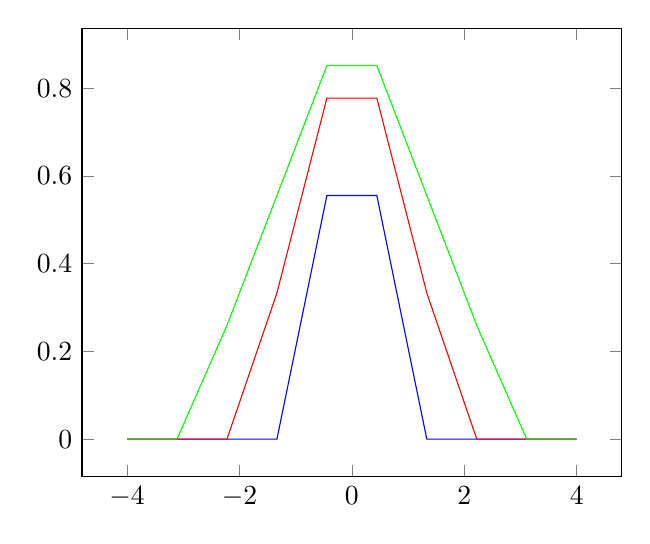
\begin{tikzpicture}
    \begin{axis}
    \addplot[domain=-4:4, samples=10, color=blue,]{max(x-1,0) + max(x+1,0) - 2*max(x,0)};
    \addplot[domain=-4:4, samples=10, color=red,]{max(x/2-1,0) + max(x/2+1,0) - 2*max(x/2,0)};
    \addplot[domain=-4:4, samples=10, color=green,]{max(x/3-1,0) + max(x/3+1,0) - 2*max(x/3,0)};
    \end{axis}
\end{tikzpicture}
    \label{fig:bump-function}
    \caption{Illustration of the so-called ``bump'' function $\psi_a(x)$ with $a = 1$ in blue, $ a = 2$ in red and $a = 3$ in green.} 
\end{figure}



\setcitestyle{numbers}
\bibliography{references}
\end{document}